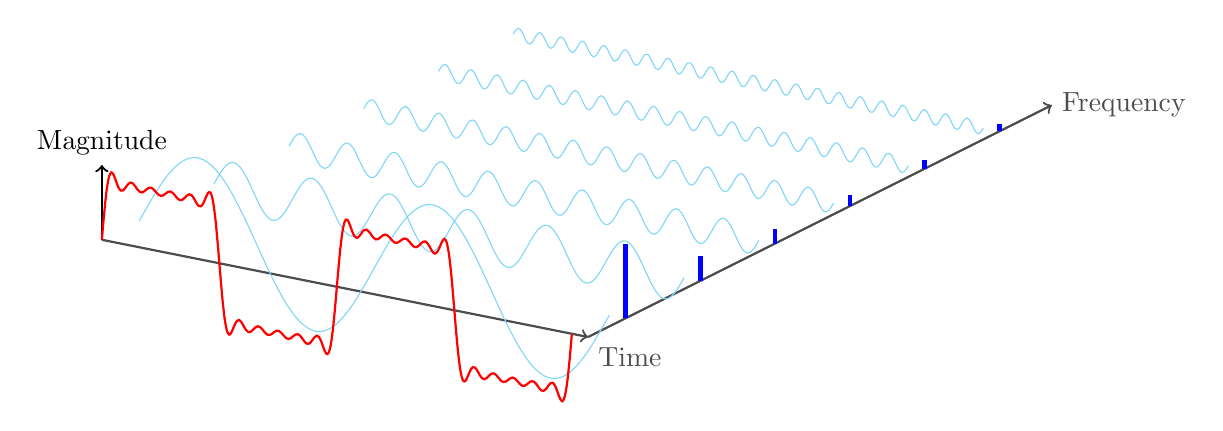
\begin{tikzpicture}[x={(1cm,0.5cm)},z={(0cm,0.5cm)},y={(1cm,-0.2cm)},scale=0.95]
    \draw[->,thick,black!70] (0,6.5,0) -- (6.2,6.5,0) node[right] {Frequency}; % 频率轴
    \draw[->,thick,black!70] (0,0,0) -- (0,6.5,0) node[below right] {Time}; % 时间轴
    \draw[->,thick] (0,0,0) -- (0,0,2) node[above] {Magnitude}; 
    
    \foreach \n in {0.5,1.5,...,5.5}{
    \draw [cyan!50, domain=0:2*pi,samples=200,smooth] 
     plot (\n,\x, {sin(4*\n*\x r)/\n });
    \draw[blue, ultra thick] (\n,6.5,0) -- (\n,6.5,1/\n);
    } % 频率逐渐增大振幅逐渐变小的正弦函数
    
    \draw [red, thick, domain=0:2*pi,samples=200,smooth] 
    plot (0,\x, {sin(4*0.5*\x r)/0.5 + sin(4*1.5*\x r)/1.5 + sin(4*2.5*\x r)/2.5 + sin(4*3.5*\x r)/3.5 + sin(4*4.5*\x r)/4.5 + sin(4*5.5*\x r)/5.5} ); 
    % 最后是手动加起来得到矩形波的逼近
\end{tikzpicture}
